\documentclass{standalone}
\usepackage[utf8]{inputenc}
\usepackage{tikz}
\usepackage{color}
\usetikzlibrary{arrows,shapes,positioning,shadows,trees}

\tikzset{
  basic/.style  = {draw, text width=3cm, drop shadow, font=\sffamily, rectangle},
  root/.style   = {basic, rounded corners=2pt, thin, align=center,
                   fill=green!60},
  level 2/.style = {basic, rounded corners=6pt, thin,align=center, fill=green!40,
                   text width=15em},
  level 3/.style = {basic, rounded corners=6pt, thin,align=center, fill=green!40,
                   text width=10em},
  level 4/.style = {basic, thin, align=left, fill=green!20, text width=10.1em}
}

\begin{document}

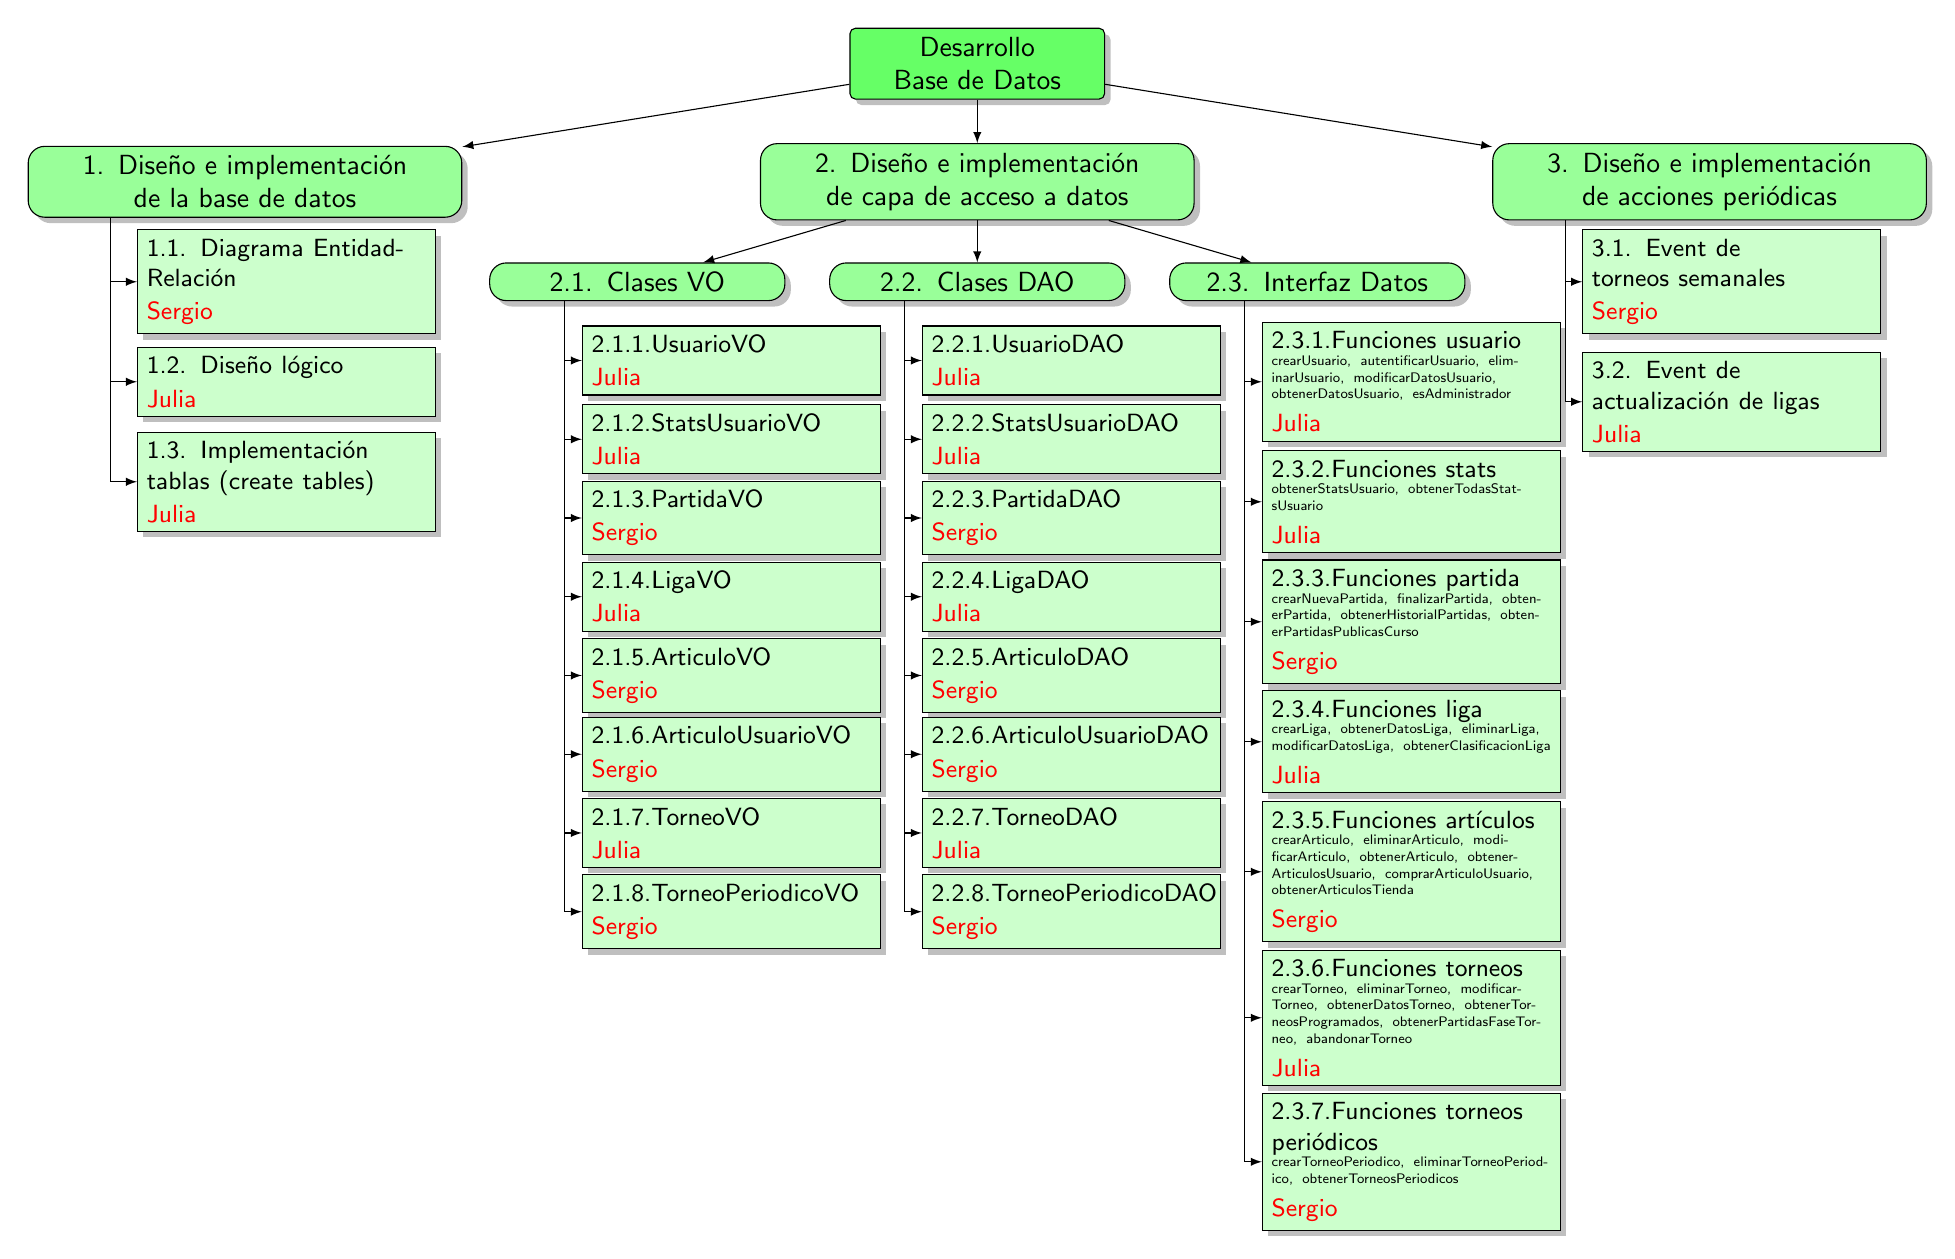
\begin{tikzpicture}[
  level 1/.style={sibling distance=93mm},
  edge from parent/.style={->,draw},
  >=latex]

% raiz inicial
\node[root] {Desarrollo Base de Datos}
% The first level, as children of the initial tree
  child {node[level 2] (c1) {1. Diseño e implementación de la base de datos}}
  child {node[level 2] (c2) {2. Diseño e implementación de capa de acceso a datos}}
  child {node[level 2] (c3) {3. Diseño e implementación de acciones periódicas}};

\begin{scope}
\node [level 3, below of = c2, node distance=0.5in] (c22) {2.2. Clases DAO};
\node [level 3, right of = c22, node distance=1.7in] (c23) {2.3. Interfaz Datos};
\node [level 3, left of = c22, node distance=1.7in] (c21) {2.1. Clases VO};
\end{scope}

% The second level, relatively positioned nodes
\begin{scope}[every node/.style={level 4}]
\node [below of = c1,node distance=0.5in, xshift=15pt] (c11) {\small{1.1. Diagrama Entidad-Relación} \\ \textcolor{red}{\small{Sergio}}};
\node [below of = c11, node distance=0.5in] (c12) {\small{1.2. Diseño lógico}\\ \textcolor{red}{\small{Julia}}};
\node [below of = c12, node distance=0.5in] (c13) {\small{1.3. Implementación tablas (create tables)} \\ \textcolor{red}{\small{Julia}}};

\node [below of = c21, xshift=34pt] (c211) {\small{2.1.1.UsuarioVO} \\ \textcolor{red}{\small{Julia}}};
\node [below of = c211] (c212) {\small{2.1.2.StatsUsuarioVO} \\ \textcolor{red}{\small{Julia}}};
\node [below of = c212] (c213) {\small{2.1.3.PartidaVO} \\ \textcolor{red}{\small{Sergio}}};
\node [below of = c213] (c214) {\small{2.1.4.LigaVO} \\ \textcolor{red}{\small{Julia}}};
\node [below of = c214] (c215) {\small{2.1.5.ArticuloVO} \\ \textcolor{red}{\small{Sergio}}};
\node [below of = c215] (c216) {\small{2.1.6.ArticuloUsuarioVO} \\ \textcolor{red}{\small{Sergio}}};
\node [below of = c216] (c217) {\small{2.1.7.TorneoVO} \\ \textcolor{red}{\small{Julia}}};
\node [below of = c217] (c218) {\small{2.1.8.TorneoPeriodicoVO} \\ \textcolor{red}{\small{Sergio}}};

\node [below of = c22, xshift=34pt] (c221) {\small{2.2.1.UsuarioDAO} \\ \textcolor{red}{\small{Julia}}};
\node [below of = c221] (c222) {\small{2.2.2.StatsUsuarioDAO} \\ \textcolor{red}{\small{Julia}}};
\node [below of = c222] (c223) {\small{2.2.3.PartidaDAO} \\ \textcolor{red}{\small{Sergio}}};
\node [below of = c223] (c224) {\small{2.2.4.LigaDAO} \\ \textcolor{red}{\small{Julia}}};
\node [below of = c224] (c225) {\small{2.2.5.ArticuloDAO} \\ \textcolor{red}{\small{Sergio}}};
\node [below of = c225] (c226) {\small{2.2.6.ArticuloUsuarioDAO} \\ \textcolor{red}{\small{Sergio}}};
\node [below of = c226] (c227) {\small{2.2.7.TorneoDAO} \\ \textcolor{red}{\small{Julia}}};
\node [below of = c227] (c228) {\small{2.2.8.TorneoPeriodicoDAO} \\ \textcolor{red}{\small{Sergio}}};

\node [below of = c23, xshift=34pt, node distance = 0.5in] (c231) {\small{2.3.1.Funciones usuario} \\ \tiny{crearUsuario, autentificarUsuario, eliminarUsuario, modificarDatosUsuario, obtenerDatosUsuario, esAdministrador}\\ \textcolor{red}{\small{Julia}}};
\node [below of = c231, node distance = 0.6in] (c232) {\small{2.3.2.Funciones stats} \\ \tiny{obtenerStatsUsuario, obtenerTodasStatsUsuario} \\ \textcolor{red}{\small{Julia}}};
\node [below of = c232, node distance = 0.6in] (c233) {\small{2.3.3.Funciones partida} \\ \tiny{crearNuevaPartida, finalizarPartida, obtenerPartida, obtenerHistorialPartidas, obtenerPartidasPublicasCurso} \\ \textcolor{red}{\small{Sergio}}};
\node [below of = c233, node distance = 0.6in] (c234) {\small{2.3.4.Funciones liga} \\ \tiny{crearLiga, obtenerDatosLiga, eliminarLiga, modificarDatosLiga, obtenerClasificacionLiga} \\ \textcolor{red}{\small{Julia}}};
\node [below of = c234, node distance = 0.65in] (c235) {\small{2.3.5.Funciones artículos} \\ \tiny{crearArticulo, eliminarArticulo, modificarArticulo, obtenerArticulo, obtenerArticulosUsuario, comprarArticuloUsuario, obtenerArticulosTienda} \\ \textcolor{red}{\small{Sergio}}};
\node [below of = c235, node distance = 0.73in] (c236) {\small{2.3.6.Funciones torneos} \\ \tiny{crearTorneo, eliminarTorneo, modificarTorneo, obtenerDatosTorneo, obtenerTorneosProgramados, obtenerPartidasFaseTorneo, abandonarTorneo} \\ \textcolor{red}{\small{Julia}}};
\node [below of = c236, node distance = 0.72in] (c237) {\small{2.3.7.Funciones torneos periódicos} \\ \tiny{crearTorneoPeriodico, eliminarTorneoPeriodico, obtenerTorneosPeriodicos} \\ \textcolor{red}{\small{Sergio}}};

\node [below of = c3, xshift=8pt, node distance = 0.5in] (c31) {\small{3.1. Event de\\ torneos semanales}\\ \textcolor{red}{\small{Sergio}}};
\node [below of = c31, node distance=0.6in] (c32) {\small{3.2. Event de \\actualización de ligas}\\ \textcolor{red}{\small{Julia}}};
\end{scope}

\foreach \value in {1,2,3}
  \draw [->] (c2) edge (c2\value);

\foreach \value in {1,2,3}
  \draw[->] (c1.195) |- (c1\value.west);

\foreach \value in {1,...,8}
  \draw[->] (c21.195) |- (c21\value.west);

\foreach \value in {1,...,8}
  \draw[->] (c22.195) |- (c22\value.west);

\foreach \value in {1,...,7}
  \draw[->] (c23.195) |- (c23\value.west);

\foreach \value in {1,...,2}
  \draw[->] (c3.195) |- (c3\value.west);
\end{tikzpicture}

\end{document}
